\documentclass{beamer}
\usepackage{graphicx} 
%Information to be included in the title page:
\usepackage[utf8]{inputenc}
\usepackage{amsmath}
\usepackage{graphicx} 
\usepackage[slovene]{babel}
\usepackage{hyperref}



\title{Carving}
\author{Gregor Kunc, Vid Jerič}
\date{2023}

\begin{document}

\frame{\titlepage}

\begin{frame}
\frametitle{Zgodovina}

\begin{figure}
    \centering
    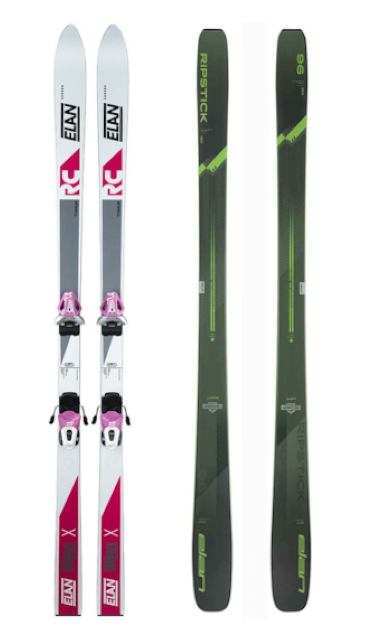
\includegraphics[scale=0.3]{../images/elan smuci.png} \\
    \caption[short]{Levo so Elan smuči iz 70-tih desno so moderne Elan smuči.}
\end{figure}

\end{frame}

\begin{frame}
    \frametitle{Tehnologija}
    
    \begin{figure}
        \centering
        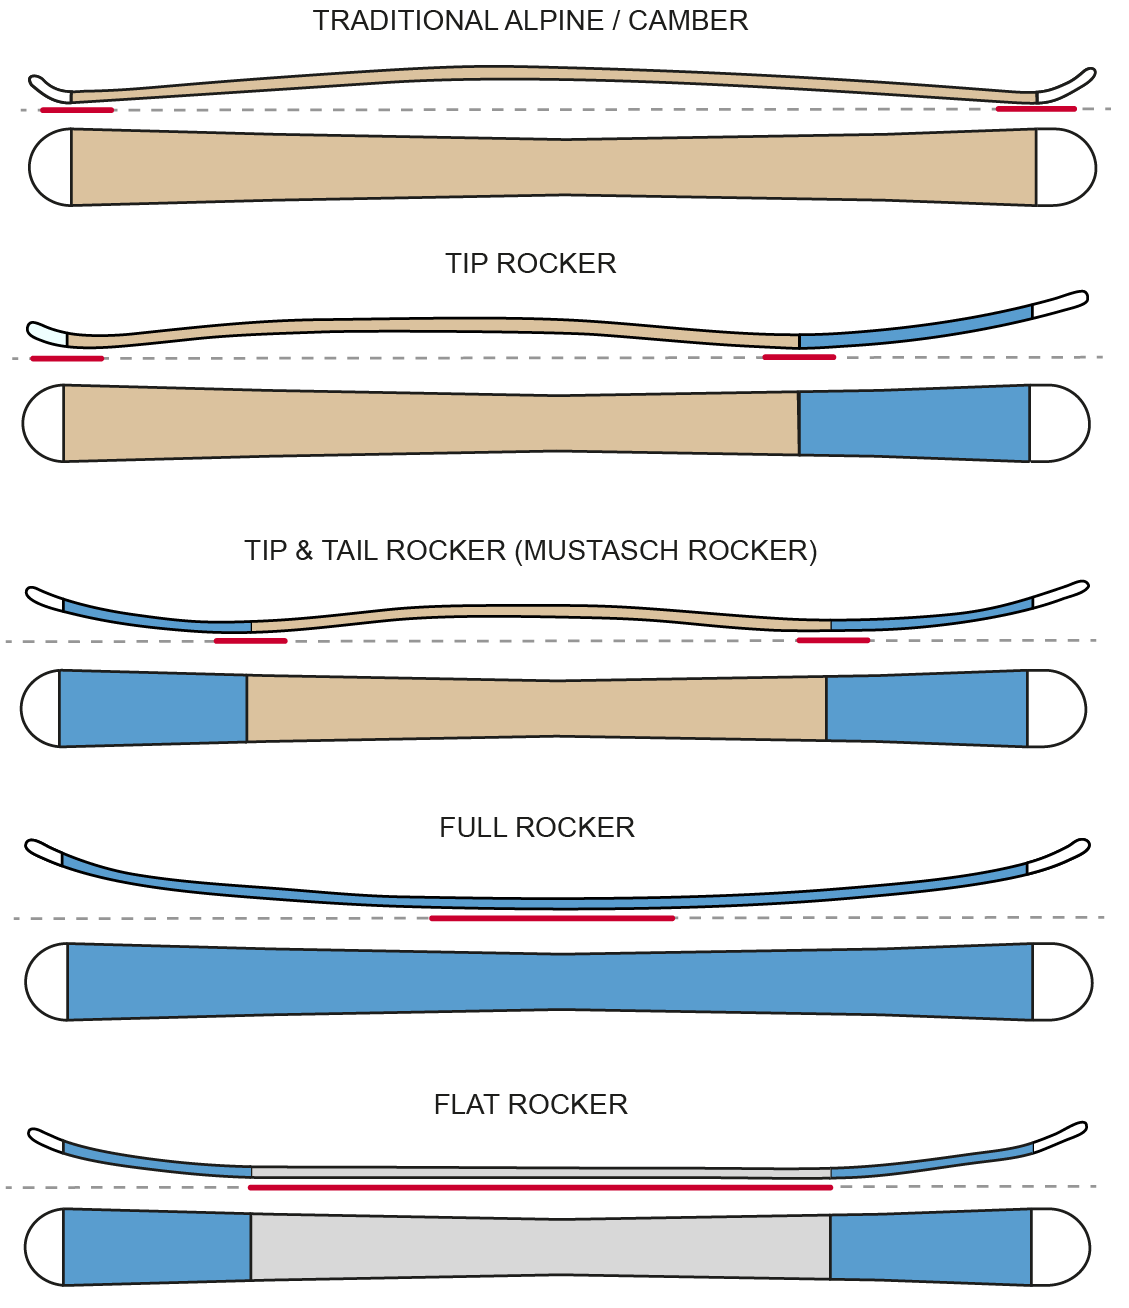
\includegraphics[scale=0.07]{../images/rocker profiles.png} \\
        \caption[short]{Različne oblike smuči, ki so posledica razvoja skozi čas.}

        \centering
        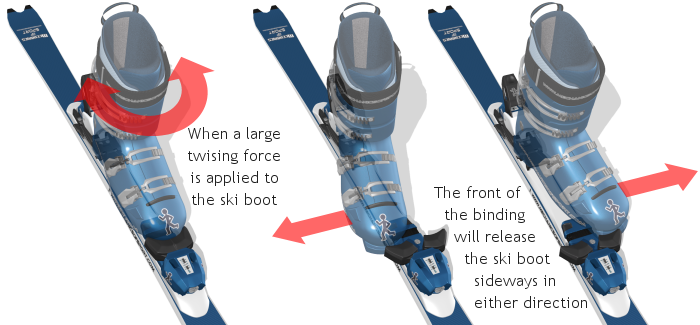
\includegraphics[scale=2]{../images/bindings-toe-release.png} \\
        \caption[short]{Sprostitveni mehanizem vezi.}

    \end{figure} 

\end{frame}

\begin{frame}
    \frametitle{Tehnika carving}
    
\begin{figure}
    \centering
    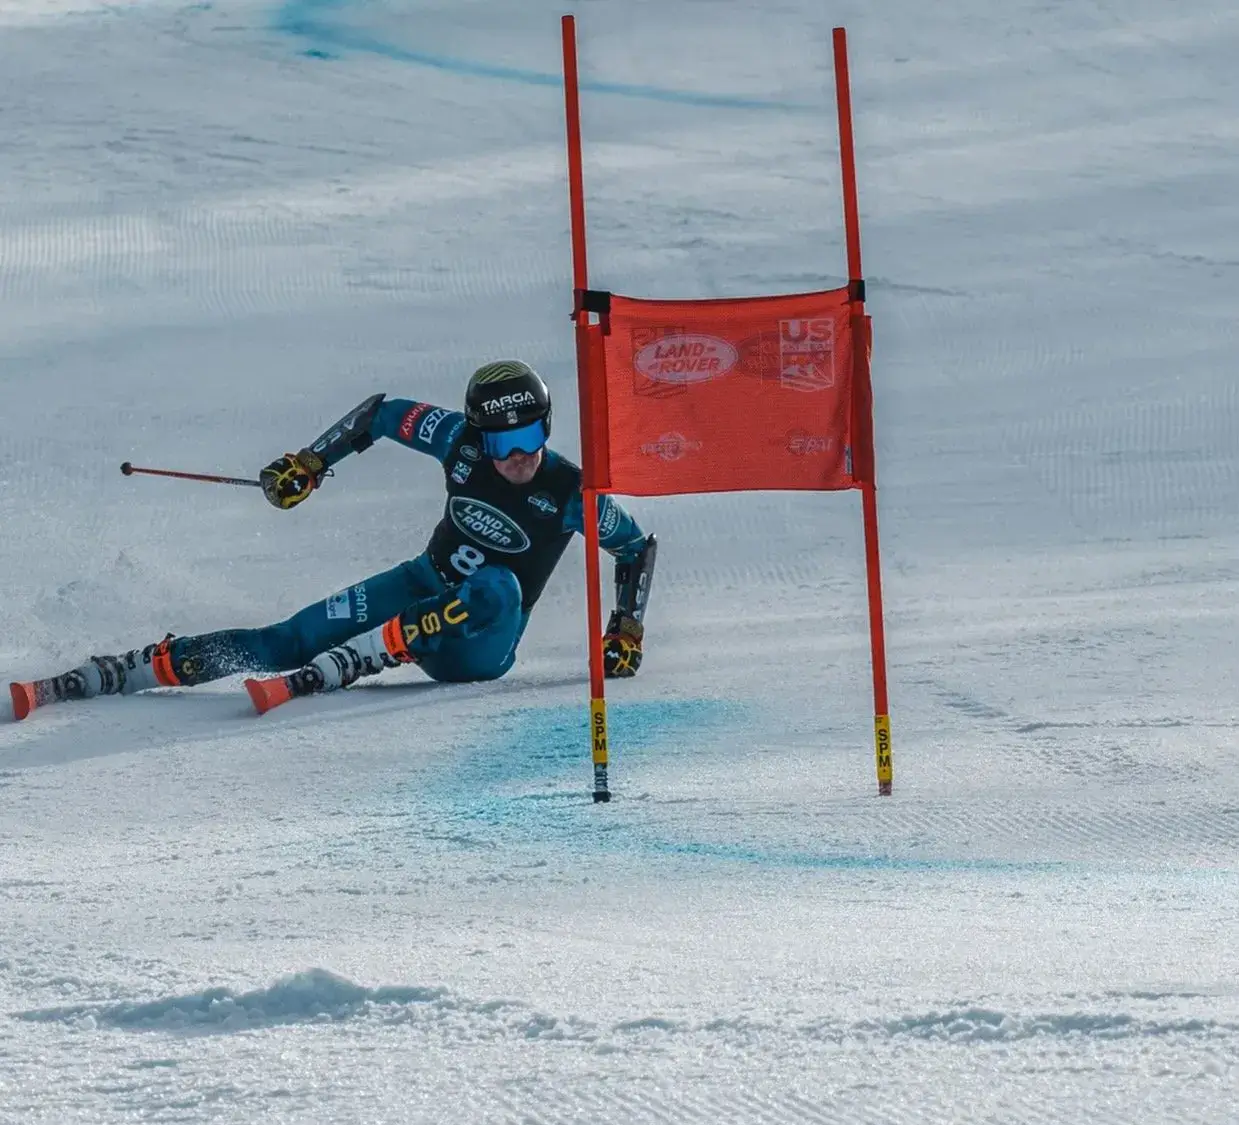
\includegraphics[scale=0.2]{../images/River-Radamus-Arcing-a-GS-turn 1.png} \\
\end{figure}

\end{frame}

\begin{frame}
    \frametitle{Podrobno}
    \begin{figure}
        \centering
        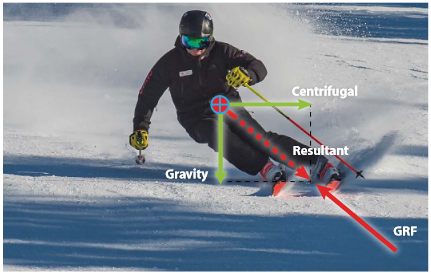
\includegraphics[scale=0.4]{../images/Screenshot 2023-12-03 152028.png} 
        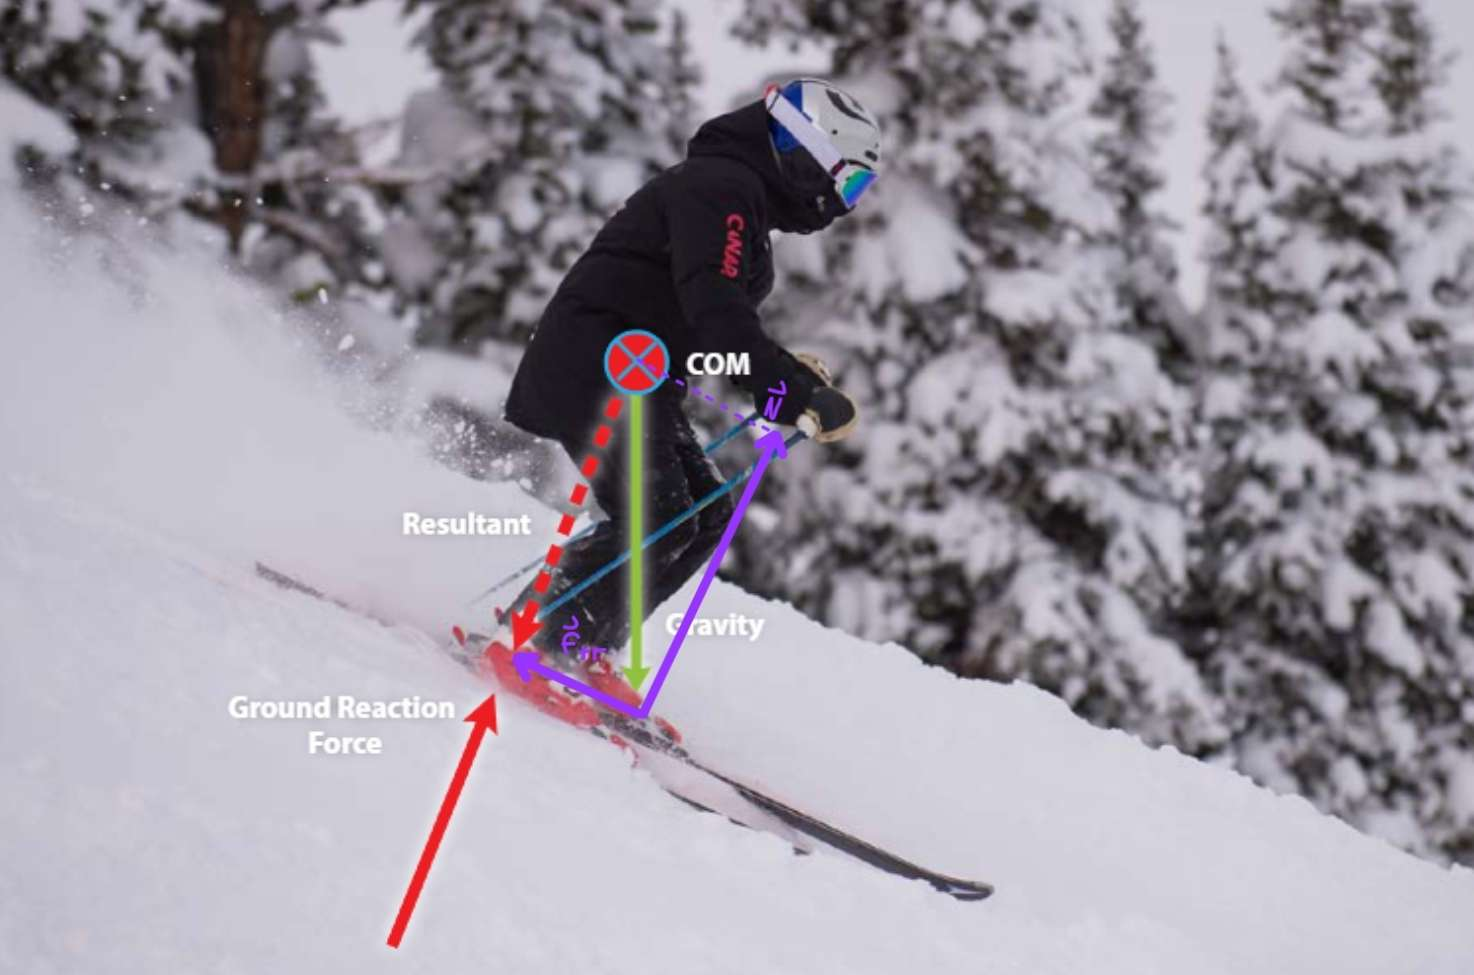
\includegraphics[scale=0.09]{../images/Sile pri com.jpg}
    \end{figure}
    \begin{figure}
        \centering
        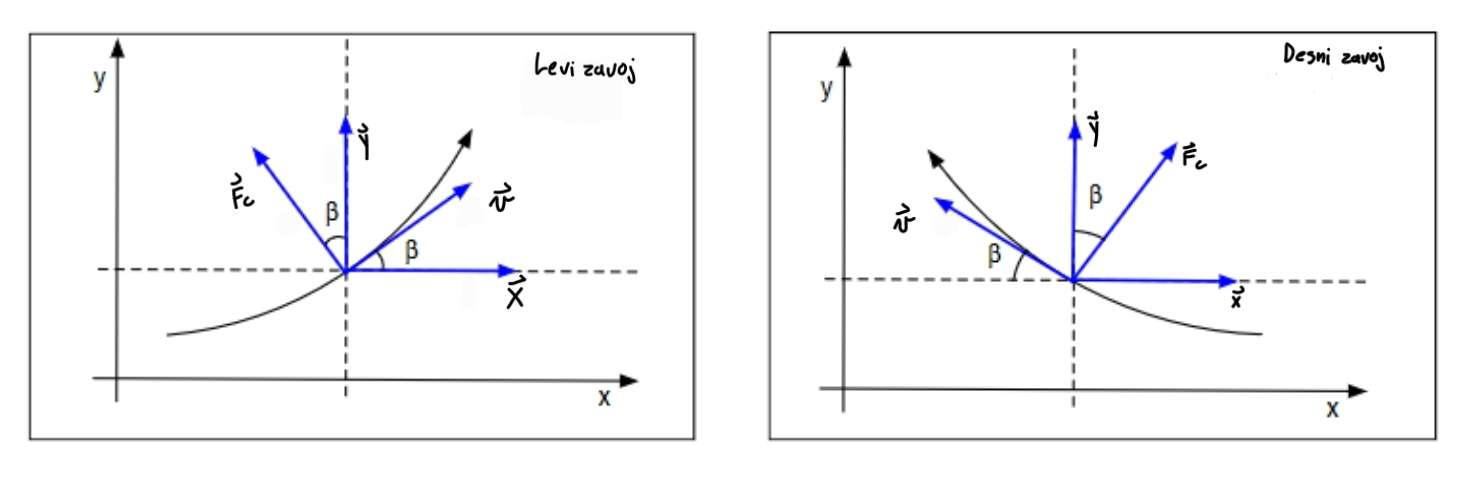
\includegraphics[scale=0.2]{../images/neke silo ovo ono.jpg} \\
    \end{figure}
\end{frame}

\begin{frame}
    \frametitle{Zanimivosti}

    \begin{figure}[h]
        \centering
        \href{https://www.youtube.com/watch?v=gz-irSJGehY}{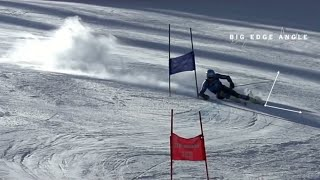
\includegraphics[width=0.8\linewidth]{../images/slika-1.jpg}}
        \label{fig:external_link}
      \end{figure}
      
\begin{figure}[h]
        \centering
        \href{https://www.youtube.com/watch?v=vM_UU11MMH0}{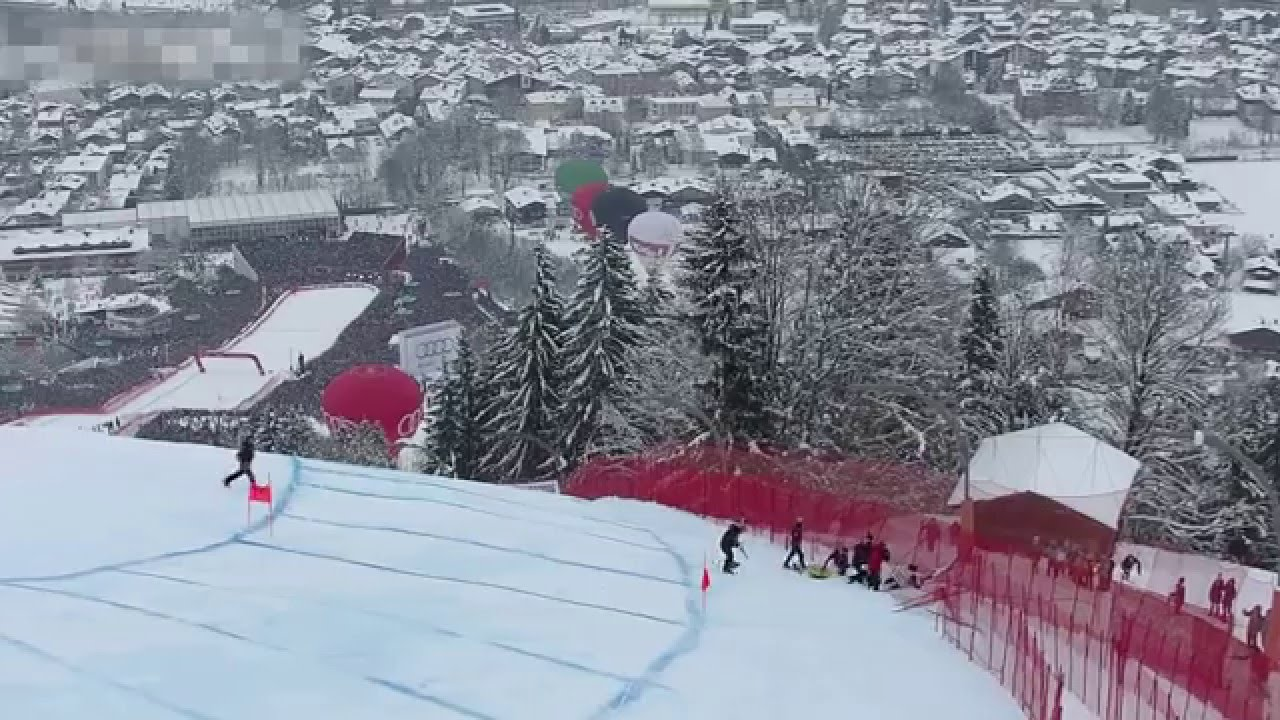
\includegraphics[width=0.8\linewidth]{../images/slika-2.jpg}}
        \label{fig:external_link}
    \end{figure}

\end{frame}

\end{document}